We can write $x(n)$ as follows:
\begin{align}
x(n) &= \sum_{k=-2}^{2}\Bigg(\frac{1}{2}\Bigg)^{\abs{k}-1}\delta[n-k]\label{ec/2005/85/eq:1}
\end{align}
where $\delta[n-k]$ is the discrete unit sample function defined as follows:
\begin{align}
\delta[n-k]=\begin{cases}
1 \text{ if } n=k\\
0 \text{ otherwise}
\end{cases}
\end{align}
From \eqref{ec/2005/85/eq:1} we have for even $n$ :
\begin{align}
y(n) &= x\Bigg(\dfrac{n}{2}-1\Bigg)\\
&= \sum_{k=-2}^{2}\Bigg(\frac{1}{2}\Bigg)^{\abs{k}-1}\delta\Bigg[\frac{n}{2}-1-k\Bigg]\\
&= \sum_{k=-2}^{2}\Bigg(\frac{1}{2}\Bigg)^{\abs{k}-1}\delta[n-2(k+1)]\label{ec/2005/85/eq:2}
\end{align}
We clearly have $y(n)$ = 0 for odd $n$ from \eqref{ec/2005/85/eq:2}. The plots of $x(n)$ and $y(n)$ are given by:
\begin{figure}[!ht]
    \centering
    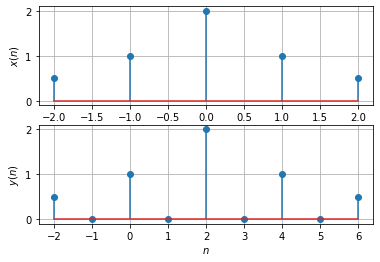
\includegraphics[width=\columnwidth] {solutions/ec/2005/85/Figures/Gate_Assignment_3_Fig_6.png}
    \caption{$x(n)$ and $y(n)$ vs $n$}
    \label{ec/2005/85/x(n) and y(n)}
\end{figure}

Hence the correct answer is option (a).
